\documentclass[11pt,oneside]{scrbook}
\usepackage[a4paper,margin=2.4cm,marginparwidth=1.8cm,marginparsep=0.4cm]{geometry}
\usepackage{../common/rlstudy}
\usepackage[ruled,vlined]{algorithm2e}

\title{{\color{rlblue}\textbf{Week 14} \\ \Huge Offline RL: Distribution Shift, Conservatism, and Implicit Q-Learning}}
\author{STUDY-RL --- a self-paced Deep RL curriculum}
\date{\today}

\begin{document}
\maketitle
\tableofcontents
\newpage

\chapter*{Learning objectives}
\addcontentsline{toc}{chapter}{Learning objectives}


% Teaching companion: a small example before the full lecture.
\noindent\textbf{Study companion.} Read \texttt{teaching\_guide.md} in this
folder for step-by-step examples, an analogy with its limits, and self-checks.
Then use \texttt{workbook.ipynb} to implement and vary the calculations.
\par\medskip

\begin{keyidea}
After this week you will be able to:
\begin{enumerate}
  \item Define the offline RL setting and explain why standard Q-learning fails on logged data
        through \emph{extrapolation error}.
  \item Derive the BCQ behaviour-support constraint and the BEAR MMD constraint from the
        Bellman backup.
  \item Reproduce the CQL conservative penalty from a min-max objective and explain its
        ``learned Q is a lower bound on $V^\pi$'' guarantee.
  \item Derive the IQL expectile value loss and the AWR/AWAC closed-form policy update.
  \item Implement IQL (tabular) and CQL on a synthetic logged GridWorld and show
        that IQL beats naive Q-learning.
  \item Estimate $V^\pi$ from a logged dataset via SNIPS and discuss the OPE-FQE-DICE tradeoffs.
  \item Translate offline RL pitfalls into concrete failure modes for recruitment matching
        deployments.
\end{enumerate}
\end{keyidea}

\chapter{Motivation \& intuition}

In every previous week the agent generated its own data: the policy that produced the
sample is the policy we are trying to improve. \marginnote{Recall: PPO, SAC, DQN all
trained from a buffer of \emph{their own} transitions.} Offline RL inverts this. We are
given a static dataset $\mathcal{D} = \{(s_i, a_i, r_i, s'_i)\}_{i=1}^N$ produced by an
unknown behaviour policy $\pi_\beta$ and must return a policy $\pi$ that performs well
in the real environment \emph{without any new interaction}.

This is the practical setting of essentially every commercial RL deployment we have
encountered: clickstreams from a recommender, broker--lead pairings logged in a CRM,
chat trajectories from a deployed assistant. The hard part is not learning per se ---
it is that the Bellman backup quietly queries actions that have \emph{never been taken
in $\mathcal{D}$}. Function approximators happily extrapolate, but in the wrong direction.

\begin{intuition}
Imagine fitting a regression on $x \in [0, 1]$ and then asking it to predict at $x = 10$.
You will get a number, but it is a fiction. Off-policy Q-learning maximises over actions:
$\max_a Q(s', a)$ pulls towards whichever $a$ happens to have the largest \emph{extrapolated}
value. The Bellman backup then propagates that fiction backward through the trajectory,
making everything worse on the next sweep. Offline RL is the discipline of \textbf{not asking}.
\end{intuition}

\begin{pitfall}
``Offline RL'' is sometimes confused with ``batch RL''. They are the same: a fixed
log, no fresh rollouts. The \emph{name} ``offline'' is to emphasise the deployment
constraint --- you cannot try a new candidate broker just to learn from the click.
\end{pitfall}

\chapter{Mathematical formulation}

\begin{definition}[Offline RL problem]
Given $\mathcal{D} = \{(s_i, a_i, r_i, s'_i)\}_{i=1}^N$ drawn from $d^{\pi_\beta}$,
discount $\gamma \in (0,1)$, and an MDP $(\States,\Actions,P,R)$ that the learner
\emph{cannot query}, find a policy $\pi: \States \to \Delta(\Actions)$ that
maximises $J(\pi) = \E_{s_0 \sim \rho_0}[\Vfn^\pi(s_0)]$.
\end{definition}

\begin{definition}[Distribution shift]
Let $d^\pi(s,a) = (1-\gamma)\sum_{t \geq 0}\gamma^t \Prb(s_t=s, a_t=a \mid \pi)$ be the
discounted occupancy. \emph{Distribution shift} is the divergence between $d^{\pi_\beta}$
(coverage in the data) and $d^\pi$ (states the learner would visit), measured by
$D_\TV$, $D_\KL$, or $\chi^2$.
\end{definition}

\section{Extrapolation error}

Define the true optimality Bellman backup
\[
  \mathcal{B}^* Q(s,a) = r(s,a) + \gamma \E_{s' \sim P}\bigl[\max_{a' \in \Actions} Q(s', a')\bigr].
\]
The action $a'$ realising the maximum may be \emph{out-of-distribution} with respect
to $\pi_\beta(\cdot \mid s')$. Under a function approximator with capacity $\theta$,
the gradient $\nabla_\theta Q(s', a')$ ``moves'' the learned $Q$ everywhere that the
network thinks $a'$ looks like another action. We get a cascading optimistic bias.

\begin{theorem}[Bellman backup error decomposition --- Fujimoto et al.\ 2019]
For any $Q$ and any state--action $(s,a)$, write the true
policy-evaluation operator as $\mathcal{B}^\pi$ and its empirical estimate
as $\hat{\mathcal{B}}^\pi$. Then
\begin{align*}
 |Q(s,a)-Q^\pi(s,a)|
 &\le |Q(s,a)-\hat{\mathcal{B}}^\pi Q(s,a)| \\
 &\quad+|(\hat{\mathcal{B}}^\pi-\mathcal{B}^\pi)Q(s,a)| \\
 &\quad+\gamma\,\E_{s'\sim P,a'\sim\pi}[|Q(s',a')-Q^\pi(s',a')|].
\end{align*}
\end{theorem}

\begin{proof}[Sketch]
Insert and subtract both the empirical backup $\hat{\mathcal{B}}^\pi Q$ and true backup $\mathcal{B}^\pi Q$
and use the $\gamma$-contraction of $\mathcal{B}^\pi$.
\end{proof}

The first term is an empirical residual; the second is model or sampling error. Neither is controlled on unsupported state--action pairs. The propagated-error term \emph{integrates over $\pi$}, including
on out-of-support actions. The whole offline literature is methods that keep
$a' \sim \pi$ close enough to $\pi_\beta$ that propagated error remains controllable.

\section{BCQ and BEAR --- behaviour regularisation}

BCQ (Fujimoto 2019) trains a conditional VAE $G_\omega(a \mid s)$ on $\mathcal{D}$ and only
considers actions sampled from $G_\omega$ plus a small perturbation network
$\xi_\phi(s, a)$:
\[
  \pi_{\mathrm{BCQ}}(s) = \argmax_{a_i + \xi_\phi(s, a_i): a_i \sim G_\omega(\cdot \mid s)} Q_\theta(s, a_i).
\]
BEAR replaces the constraint by a sampled MMD divergence
$\mathrm{MMD}^2(G_\omega(\cdot|s), \pi(\cdot|s)) \le \varepsilon$, enforced via a
Lagrangian penalty on the actor.

\section{CQL --- conservative Q-learning}

\begin{definition}[CQL objective, discrete actions]
For a parameter $\alpha > 0$,
\begin{align*}
  \mathcal{L}_{\mathrm{CQL}}(\theta) &= \alpha \, \E_{s \sim \mathcal{D}}\!\bigl[\log \textstyle\sum_a \exp Q_\theta(s,a) - \E_{a \sim \pi_\beta(\cdot|s)} Q_\theta(s,a)\bigr] \\
  &\quad + \tfrac{1}{2}\, \E_{(s,a,r,s') \sim \mathcal{D}}\!\bigl[(Q_\theta(s,a) - \mathcal{B}^\pi \hat{Q}(s,a))^2\bigr].
\end{align*}
\end{definition}

\begin{remark}[Conservatism: intuition versus guarantee]
Kumar et al.\ (2020) establish policy-value lower bounds for specified CQL
policy-evaluation variants under their tabular, coverage, sampling-error, and
regularisation conditions. This is not a pointwise guarantee for every learned
$Q(s,a)$, every penalty coefficient, or an arbitrary neural optimiser.
\end{remark}

\paragraph{Penalty-gradient derivation (not a lower-bound proof).}
At a fixed state let $b_a$ be the empirical behaviour frequency, $y_a$ a
frozen Bellman target, and $\mu_a=\exp Q_a/\sum_j\exp Q_j$. The statewise objective is
\[
 \ell(Q)=\alpha[\log\sum_a e^{Q_a}-\sum_a b_a Q_a]
       +\tfrac12\sum_a b_a(Q_a-y_a)^2.
\]
Differentiation gives
\[
 \frac{\partial\ell}{\partial Q_a}=\alpha(\mu_a-b_a)+b_a(Q_a-y_a).
\]
For $b_a>0$, stationarity implies $Q_a=y_a-\alpha(\mu_a/b_a-1)$.
The factor $b_a$ in the squared-error gradient is essential. The penalty
pushes down actions overweighted by $\mu$ relative to the log; it cannot,
by itself, prove a policy-value bound for every target policy.

\begin{pitfall}
Setting $\alpha$ too large makes the policy degenerate to imitation; too small lets
extrapolation error in. The standard recipe is to \emph{tune $\alpha$ with a
Lagrangian} on the budget $\mathcal{B}_\mathrm{CQL} = \log Z - \E_{\pi_\beta} Q \leq \tau$.
\end{pitfall}

\section{IQL --- implicit Q-learning}

IQL never explicitly samples actions from $\pi$; instead it estimates the upper
expectile of $Q(s,a)$ for $a \sim \pi_\beta$ and uses that as a value baseline.

\begin{definition}[Expectile loss]
For $\tau \in (0,1)$ and residual $u = y - \hat y$,
\[
  L_2^\tau(u) = |\tau - \mathbf{1}\{u < 0\}| \cdot u^2.
\]
The expectile is the minimiser of $\E[L_2^\tau(Y - v)]$ over $v$.
\end{definition}

\begin{theorem}[IQL value backup]
In the finite-action tabular setting with exact optimisation and bounded, fixed $Q_{\hat\theta}$, let $V_\psi$ solve $\min_\psi \E_{(s,a)\sim \mathcal{D}}[L_2^\tau(Q_{\hat\theta}(s,a) - V_\psi(s))]$.
Then for $\tau \to 1$, $V_\psi(s) \to \max_{a \in \mathrm{supp}\,\pi_\beta(\cdot|s)} Q_{\hat\theta}(s,a)$.
\end{theorem}

\begin{proof}[Sketch]
Fix $s$; we are estimating the $\tau$-expectile of the conditional distribution
of $Q(s,a)$ under $a \sim \pi_\beta(\cdot|s)$. The $\tau$-expectile of a bounded
random variable converges to its essential supremum as $\tau \to 1$. So the value
becomes the in-support max --- never the global max, which is exactly what we
wanted to avoid.
\end{proof}

\[
  \boxed{\,L_V(\psi) = \E_{\mathcal{D}}\!\bigl[L_2^\tau(Q_{\hat\theta}(s,a) - V_\psi(s))\bigr],\quad
         L_Q(\theta) = \E_{\mathcal{D}}\!\bigl[(r + \gamma V_\psi(s') - Q_\theta(s,a))^2\bigr]\,}
\]

\section{AWR / AWAC policy extraction}

Given $A(s,a) = Q(s,a) - V(s)$, AWAC solves
\[
  \pi^\star = \argmax_\pi \E_{(s,a) \sim \mathcal{D}}\!\bigl[ \log \pi(a|s) \cdot \exp(\beta A(s,a))\bigr],
\]
which is the closed-form solution of the KL-constrained policy improvement
\begin{align*}
  \max_\pi &\; \E_{s \sim \mathcal{D}, a \sim \pi}[A(s,a)] \\
  \text{s.t.}\; & \KL(\pi(\cdot|s) \,\|\, \pi_\beta(\cdot|s)) \le \varepsilon.
\end{align*}
The Lagrangian is $A(s,a) - (1/\beta) \log(\pi/\pi_\beta) + \lambda$. Setting the
derivative w.r.t.\ $\pi(a|s)$ to zero gives $\pi^\star(a|s) \propto \pi_\beta(a|s) \exp(\beta A(s,a))$;
because $\pi_\beta$ is the empirical distribution of actions in $\mathcal{D}$, the
maximum-likelihood policy regression on weighted samples is the same fit.

\begin{figure}[h]
\centering
\begin{tikzpicture}
  \draw[thick, rlblue] (0,0) -- (5.6, 0);
  \node[below] at (0,-0.05) {$\pi_\beta$};
  \node[below] at (5.6,-0.05) {$\pi^\star$};
  \draw[->, thick, rlteal] (0.3,0.5) .. controls (2.5, 2.2) and (4.0, 2.2) .. (5.3, 0.5);
  \node[rlteal, above] at (3, 2.2) {AWR: $\propto \exp(\beta A)$};
  \draw[<->, thick, dashed, rlorange] (0.3,-0.6) -- (5.3, -0.6);
  \node[rlorange, below] at (3, -0.6) {KL budget $\varepsilon$};
\end{tikzpicture}
\caption{AWR/AWAC: stay inside a KL ball of $\pi_\beta$, reweight by exponentiated advantage.}
\end{figure}

\section{TD3+BC and ReBRAC}

TD3+BC is a one-line change to TD3: add $\lambda \, \|\pi(s) - a\|_2^2$ to the actor loss,
with $\lambda$ inversely proportional to $|Q|$. ReBRAC tightens this with a higher
discount, layer-norm critics, and per-step BC weight tuned via $\E[Q]$ normalisation,
producing the strongest non-transformer offline scores on D4RL as of 2024.

\section{Off-policy evaluation (OPE) primer}

Let $\pi$ be a target policy and $\pi_\beta$ the behaviour policy. The
\textbf{importance-sampling} estimator of $V^\pi$ is
\[
  \hat V^\pi_{\mathrm{IS}} = \frac{1}{n} \sum_{i=1}^n \rho_i \, G_i,
  \qquad \rho_i = \prod_{t=0}^{T_i-1} \frac{\pi(a_t \mid s_t)}{\pi_\beta(a_t \mid s_t)}.
\]
The variance scales exponentially with $T$ --- the ``curse of horizon''.
\textbf{Self-normalised IS (SNIPS)} replaces the $1/n$ by $1/\sum_i \rho_i$, biased but
much lower variance. \textbf{FQE} (Fitted-Q Evaluation) is the model-based cousin:
fit $Q^\pi$ by repeated Bellman regression on $\mathcal{D}$. \textbf{DICE} family
(DualDICE, GenDICE) estimates the stationary density ratio $d^\pi / d^{\pi_\beta}$
directly via a Fenchel dual, giving stable estimates that do not depend on horizon.

\begin{pitfall}
SNIPS with deterministic target policies is degenerate: $\rho_i$ is either zero or
$\prod 1/\pi_\beta$, so most episodes get zero weight. Soft (epsilon-mixed) target
policies are mandatory for IS estimators on offline data.
\end{pitfall}

\chapter{Algorithms}

\begin{algorithm}[H]
\caption{IQL --- Implicit Q-Learning}
\KwIn{Dataset $\mathcal{D}$, expectile $\tau$, AWR temperature $\beta$,
      learning rates $\eta_v, \eta_q, \eta_\pi$.}
Initialise $V_\psi, Q_\theta, Q_{\hat\theta} \leftarrow Q_\theta, \pi_\phi$\;
\For{$t = 1, \ldots, T$}{
  Sample minibatch $\{(s_i, a_i, r_i, s'_i)\}_{i=1}^B \sim \mathcal{D}$\;
  $\psi \leftarrow \psi - \eta_v \nabla_\psi \tfrac{1}{B}\sum_i L_2^\tau(Q_{\hat\theta}(s_i,a_i) - V_\psi(s_i))$\;
  $\theta \leftarrow \theta - \eta_q \nabla_\theta \tfrac{1}{B}\sum_i (r_i + \gamma V_\psi(s'_i) - Q_\theta(s_i,a_i))^2$\;
  $\phi \leftarrow \phi - \eta_\pi \nabla_\phi -\tfrac{1}{B}\sum_i \exp(\beta (Q_{\hat\theta}(s_i,a_i) - V_\psi(s_i))) \cdot \log \pi_\phi(a_i|s_i)$\;
  Soft-update $\hat\theta \leftarrow (1-\rho)\hat\theta + \rho\theta$\;
}
\end{algorithm}
\textbf{Complexity:} $O(B \cdot |\theta|)$ per step. Three networks; trains 5--10$\times$
faster than CQL because no Q-on-OOD sampling.

\section{Worked numerical example}

Take a two-state, two-action MDP. $s \in \{s_0, s_1\}$, $a \in \{0, 1\}$,
deterministic transitions $s_0 \xrightarrow{a} s_a$, terminal at $s_1$ with reward $+1$
on entry, step reward $-0.1$ on $s_0 \to s_0$. Logger gives $a=1$ (good action) 70\% and
$a=0$ 30\%. $\gamma = 0.9$.

True values: $Q^\star(s_0, 0) = -0.1 + 0.9 \cdot Q^\star(s_0,1) = -0.1 + 0.9 = 0.8$;
$Q^\star(s_0, 1) = 1.0$. With $\tau = 0.7$, the expectile $V_\psi(s_0)$
minimises $0.3(1-0.7)(V-0.8)^2+0.7(0.7)(1-V)^2$ for $0.8<V<1$, giving
$V_\psi(s_0) = (0.09\cdot0.8+0.49\cdot1)/(0.09+0.49) = 0.96897$, above the logger-weighted average $0.94$.
The AWR weights are $\exp(\beta(Q-V)) = (\exp(-0.16897 \beta), \exp(0.03103 \beta))$, so for
$\beta=3$, the relative weight of $a=1$ vs $a=0$ is $\exp(0.6) \approx 1.82$ --- the
relative action probability also includes the logger odds: $(0.7/0.3)\exp(0.6)\approx4.25$. A fixed temperature is a penalty choice, not a verified hard KL budget. This calculation holds $Q=Q^\star$ fixed; the coupled IQL fixed point need not equal $Q^\star$.

\chapter{Implementation walkthrough}

The tabular IQL agent (see \texttt{project/agent.py}) has 25 states and 4 actions, so
$Q \in \Real^{25 \times 4}$ and $V \in \Real^{25}$.

\begin{codebox}
\begin{minted}{python}
def expectile_loss_grad(u, tau):
    w = np.where(u < 0, 1.0 - tau, tau)
    return w * u

# in IQLAgent.update_value:
u = self.Q[s_idx, a] - self.V[s_idx]
grad = expectile_loss_grad(u, self.tau)
for s, g in zip(s_idx, grad):
    self.V[s] += self.lr_v * g
\end{minted}
\end{codebox}

The CQL update applies the standard Bellman step \emph{and} a per-state penalty
gradient $\mathrm{softmax}(Q(s,\cdot)) - \mathbf{e}_{a_\beta}$ scaled by $\alpha$:

\begin{codebox}
\begin{minted}{python}
qs = self.Q[s]
p = np.exp(qs - qs.max()); p /= p.sum()
grad_pen = p.copy(); grad_pen[a_beta] -= 1.0
self.Q[s] -= self.lr_q * self.alpha * grad_pen
\end{minted}
\end{codebox}

The dataset comes from \texttt{collect\_logged\_dataset} which mixes an
$\varepsilon$-greedy logger ($\varepsilon = 0.3$) with 20\% pure-random episodes ---
imitating a noisy real-world logger.

\chapter{Empirical results}

\begin{figure}[h]
\centering
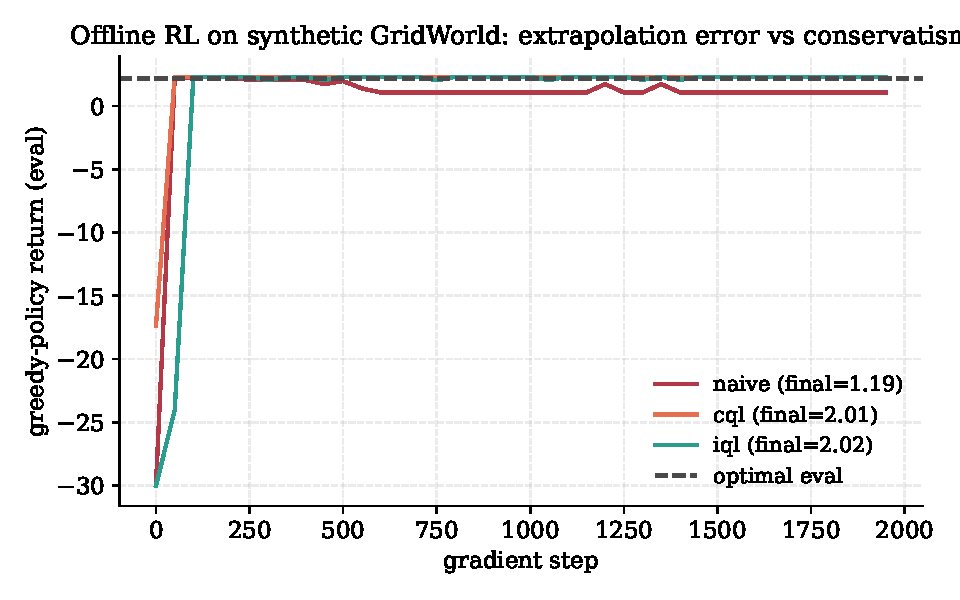
\includegraphics[width=0.9\textwidth]{figs/fig_offline_curves.pdf}
\caption{Greedy-policy evaluation return on the 5$\times$5 GridWorld. The dashed
line evaluates the dynamic-programming policy on 100 episodes. Curves use 200
logged episodes, 2000 updates, and one seed; their ordering is an empirical
observation, not a guarantee of any offline algorithm.}
\end{figure}

\begin{figure}[h]
\centering
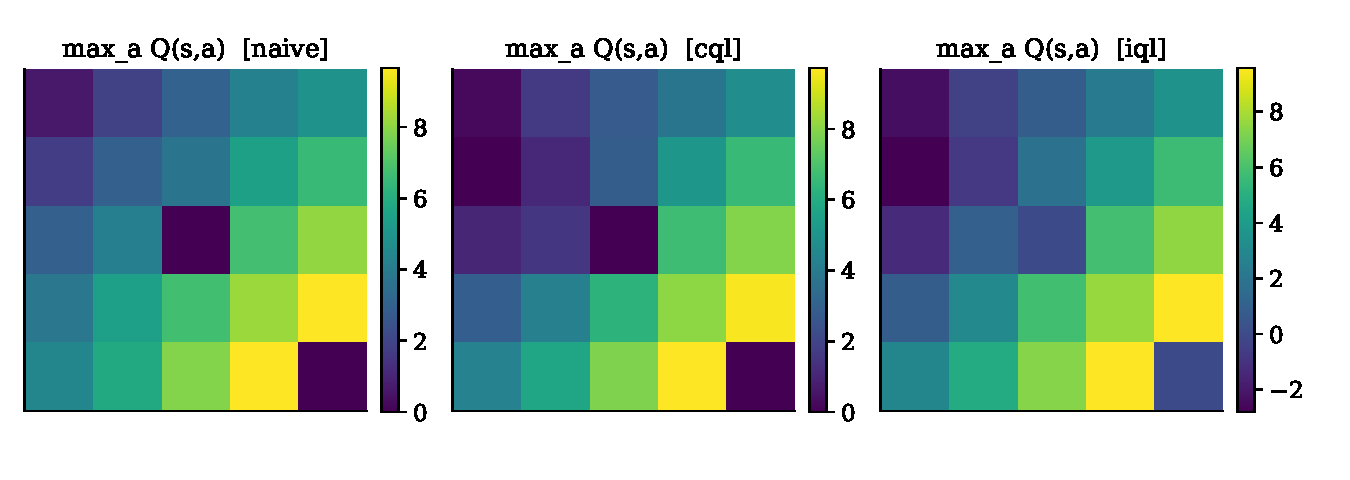
\includegraphics[width=\textwidth]{figs/fig_q_heatmaps.pdf}
\caption{Learned $\max_a Q(s,a)$ heatmaps. These show fitted scores, without an
independent pointwise error comparison or a certified CQL lower bound.}
\end{figure}

\begin{safetyangle}
\textbf{Distribution-shift failure modes for offline RL in production.}
\begin{enumerate}
  \item \textbf{Silent extrapolation.} A naive Q-learner trained on broker--lead logs
        will happily score lead--broker pairs that never co-occurred. There is no
        ``I don't know'' signal; the lift looks plausible until the policy is shipped.
  \item \textbf{Logger drift.} The behaviour policy in production changes over time
        (new business rules, new brokers). The IS estimator becomes biased the moment
        $\pi_\beta$ is non-stationary and the deployment cycle is slow.
  \item \textbf{Mitigations.}
        \begin{enumerate}[label=(\alph*)]
          \item Always run an FQE or SNIPS estimate as a \emph{guard} before shipping;
                refuse to deploy if the estimate has confidence-interval width
                $>$ 20\% of the median.
          \item Constrain the deployment policy to the \emph{support} of $\pi_\beta$
                via a sample-from-VAE constraint (BCQ) or an explicit KL penalty (AWAC).
          \item Maintain a fresh ``exploration channel'' (a small $\varepsilon$ of
                random routing) so the dataset coverage never collapses.
        \end{enumerate}
\end{enumerate}
Citations: \textsc{Levine et al.\ 2020, arXiv:2005.01643} (tutorial);
\textsc{Kumar et al.\ 2020, NeurIPS} (CQL).
\end{safetyangle}

\begin{matching}
\textbf{Recruitment matching from logs.} An ATS like synthetic ATS accumulates a vast log
of recruiter--candidate--outcome tuples: $(c_i, j_i, a_i \in \{\mathrm{reject},
\mathrm{phone},\mathrm{onsite},\mathrm{offer}\}, r_i)$. These were generated by a mixture
behaviour policy --- a blend of human recruiters using various heuristics. Naive
training of a ranker on this with online RL would extrapolate to candidates the
recruiters never advanced. IQL is the right hammer: train $V(c,j)$ on \emph{the
expectile of recruiter outcomes} and extract a soft ranker via AWR. The conservatism
of $V$ at $\tau \approx 0.8$ tracks ``best plausible recruiter outcome'' instead of
``best imagined outcome''. The KL constraint then bounds how aggressively the
suggested ranking can deviate from what recruiters historically did --- crucial for
both EEOC explainability and for keeping the change manageable in production.
\end{matching}

\chapter{Exercises}

See \texttt{workbook.ipynb} for the graded, hint-enriched versions.
\begin{itemize}
  \item \textbf{Ex.\ 1 ($\star$)} Derive and plot the expectile loss for $\tau \in \{0.5, 0.7, 0.9\}$.
  \item \textbf{Ex.\ 2 ($\star$)} Compute AWR weights for a given advantage vector.
  \item \textbf{Ex.\ 3 ($\star$$\star$)} Derive the CQL penalty gradient w.r.t.\ a single $Q(s,a)$.
  \item \textbf{Ex.\ 4 ($\star$$\star$)} Build the logged dataset and inspect coverage.
  \item \textbf{Ex.\ 5 ($\star$$\star$)} Train IQL; visualise the learned policy.
  \item \textbf{Ex.\ 6 ($\star$$\star$)} CQL ablation over $\alpha \in \{0.1, 1, 10\}$.
  \item \textbf{Ex.\ 7 ($\star$$\star$$\star$)} SNIPS off-policy evaluation against an $\varepsilon$-smoothed greedy target.
  \item \textbf{Ex.\ 8 ($\star$$\star$$\star$, meaningful objective)} Apply IQL to a tiny recruiter--candidate
        logged dataset (simulated) and produce a ranked candidate list per job.
\end{itemize}

\chapter{Further reading}

See \texttt{extended\_reading.pdf} for annotated discussions of Levine et al.\ 2020
(offline RL tutorial), Kumar et al.\ 2020 (CQL), Kostrikov et al.\ 2021 (IQL),
Tarasov et al.\ 2023 (ReBRAC), and the OPE survey by Voloshin et al.\ 2021.
Sourced from \texttt{research/offline\_modelbased\_sota.md}.

\end{document}
